\documentclass[a4paper]{article}
\usepackage{amsmath,amssymb,caption,enumitem,float,geometry,graphicx,indentfirst,minted,parskip,tabularx,xcolor}
\usepackage{float}
\captionsetup[figure]{labelsep=period}
% \captionsetup[table]{labelsep=period}
\definecolor{bg}{rgb}{0.95,0.95,0.95}
\geometry{left=3.5cm,right=3.5cm,top=3.3cm,bottom=3.3cm}
\setlength{\parindent}{2em}
\usemintedstyle{emacs}
\begin{document}
\begin{titlepage}
    \vspace*{0.25cm}
    \noindent\rule[0.25\baselineskip]{\textwidth}{1pt}
    \begin{center}
        \huge{\textsc{UM--SJTU Joint Institute}}\vspace{0.3em}\\
        \huge{\textbf{System-on-Chip Design (ECE4810J)}}\vspace{0.3em}\\
        \noindent\rule[0.25\baselineskip]{\textwidth}{1pt}
    \end{center}
    \begin{center}
        \vspace{5cm}
        \Large{\textsc{Laboratory Report}}\vspace{0.5em}\\
        \Large{\textbf{Lab 1. Getting Started with Arty Z7 SoC development platform}}\vspace{1em}\\
        \Large{\textbf{Group 2}}\\
    \end{center}
    \vfill
    \large
    \begin{tabular}{ll}
        Name: Haochen Wu \hspace*{2em}&ID: 518021910558\hspace*{2em}\\
        Name: Yihua Liu \hspace*{2em}&ID: 518021910998\hspace*{2em}\\
        Name: Siyuan Zhang \hspace*{2em}&ID:
        518370910180 \hspace*{2em}\\
        \\
        Date: \today
    \end{tabular}
\end{titlepage}
\tableofcontents
\newpage
\section{Introduction}
In this project, we gain the basic knowledge of the Vivado and Vitis environment. We practice to build a basic Zynq system on the Arty Z7-20 SoC. And we learn to create custom IP blocks at RTL level using Verilog.

\section{Part3: Building a basic ZYNQ system on the Arty Z-7 board}
In this part, we add the Zynq PS into a Vivado design, so that this hardware design can be exported to Vitis as a platform where we can run software program. Here of some screen shots related to part 3 in lab manual.
\begin{figure}[H]
    \centering
    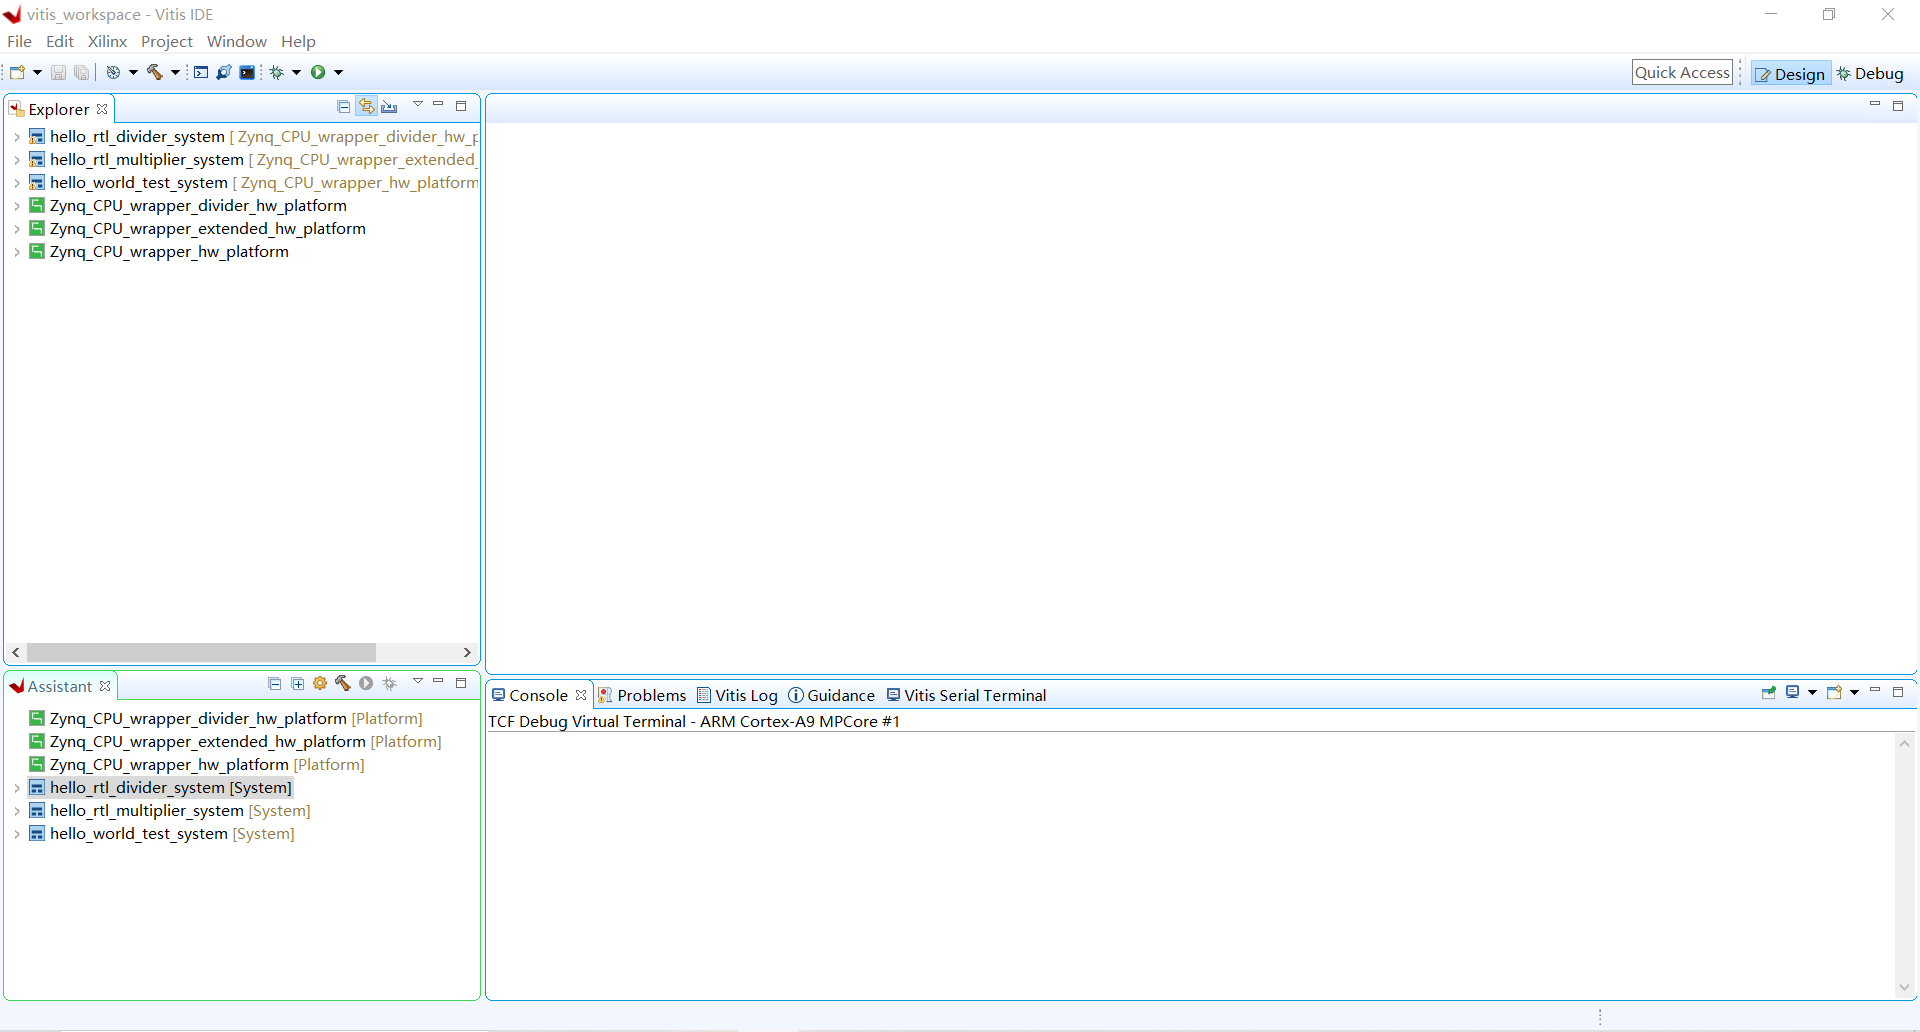
\includegraphics[width=14cm]{1}
    \caption{Eclipse environment}
    \label{fig:1}
\end{figure}

\begin{figure}[H]
    \centering
    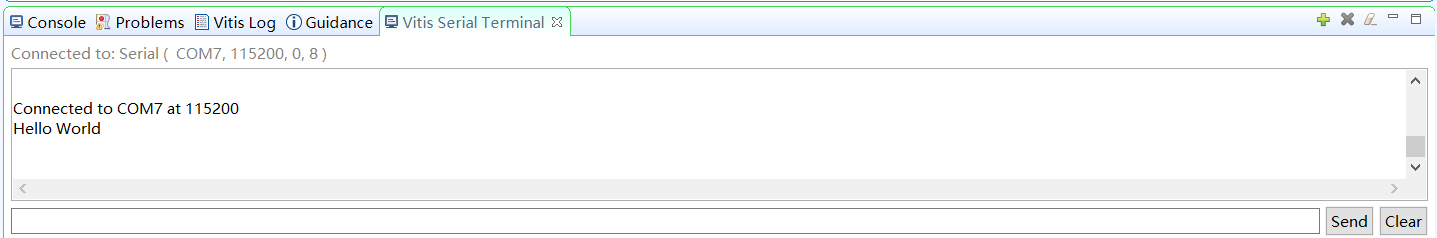
\includegraphics[width=14cm]{2_new}
    \caption{The Message Hello World in the SDK Terminal}
    \label{fig:2}
\end{figure}

\begin{figure}[H]
    \centering
    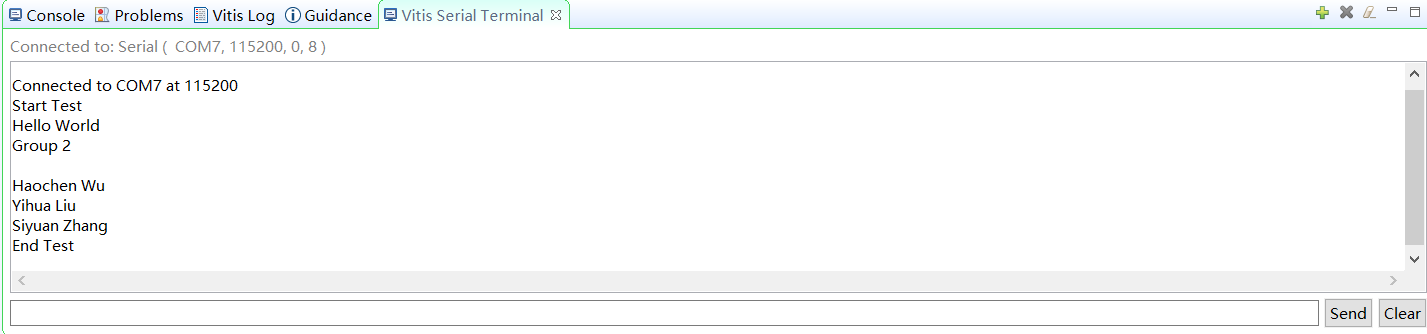
\includegraphics[width=14cm]{3_new}
    \caption{The SDK Terminal Where It Outputs Group Name and Members’ Names}
    \label{fig:3}
\end{figure}
%\\\hspace*{\fill}\\

\begin{figure}[H]
    \centering
    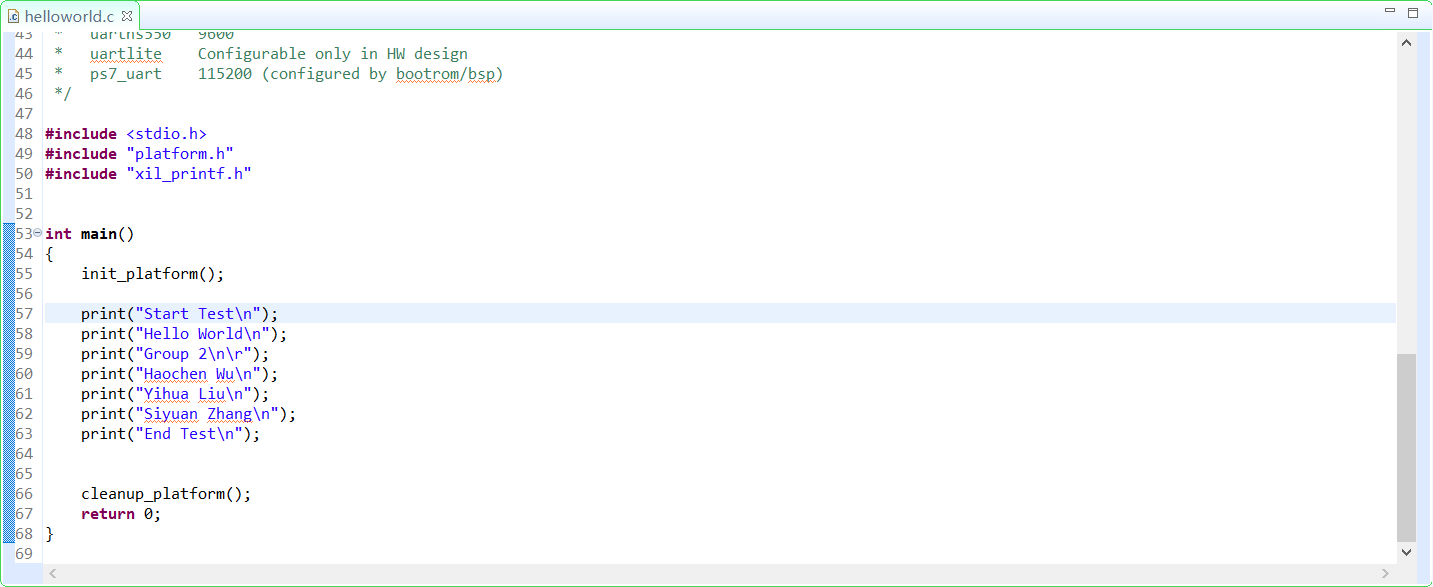
\includegraphics[width=14cm]{4}
    \caption{The Modified C Code}
    \label{fig:4}
\end{figure}
The screenshot of modified C code is shown above. The code file is submitted together with this report in the zip package.
\section{Part4: Creating and using custom IP blocks in Verilog}
In this part, we firstly add a multiplier as a IP block into the system. Secondly, we create our own divider, which computes the qoutient and remainder of two 16-bit numbers, add this new IP block, and connect it to Zynq PS via AXI interface. Here of some screen shots related to part 4 in lab manual.
\begin{figure}[H]
    \centering
    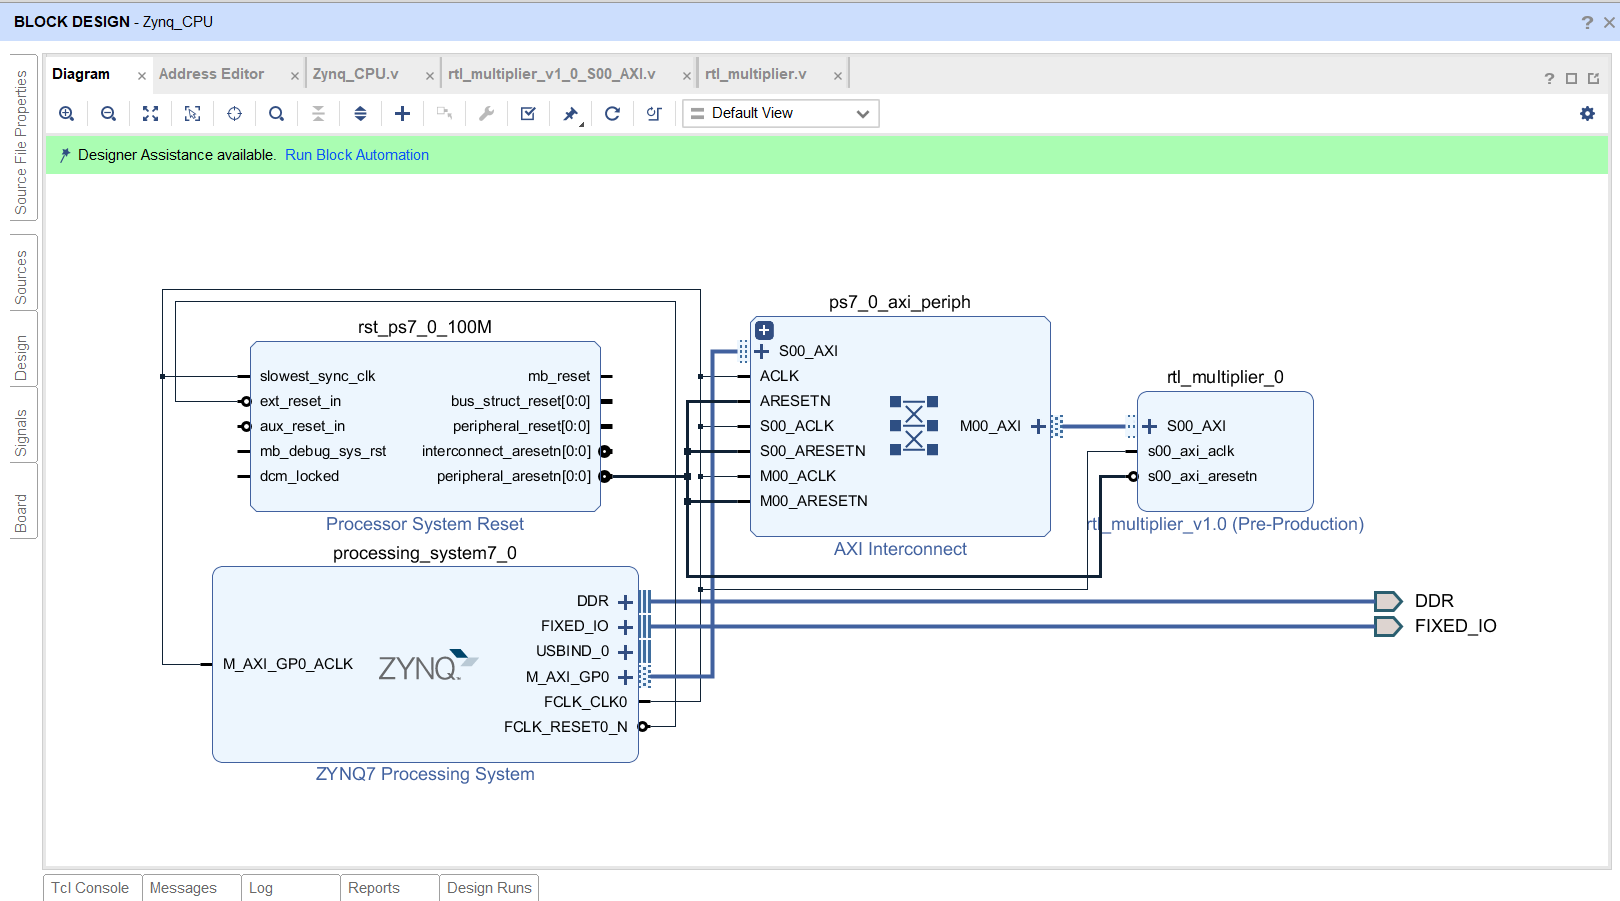
\includegraphics[width=14cm]{5_new.png}
    \caption{Screenshot of the Multiplier}
    \label{fig:5}
\end{figure}

\begin{figure}[H]
    \centering
    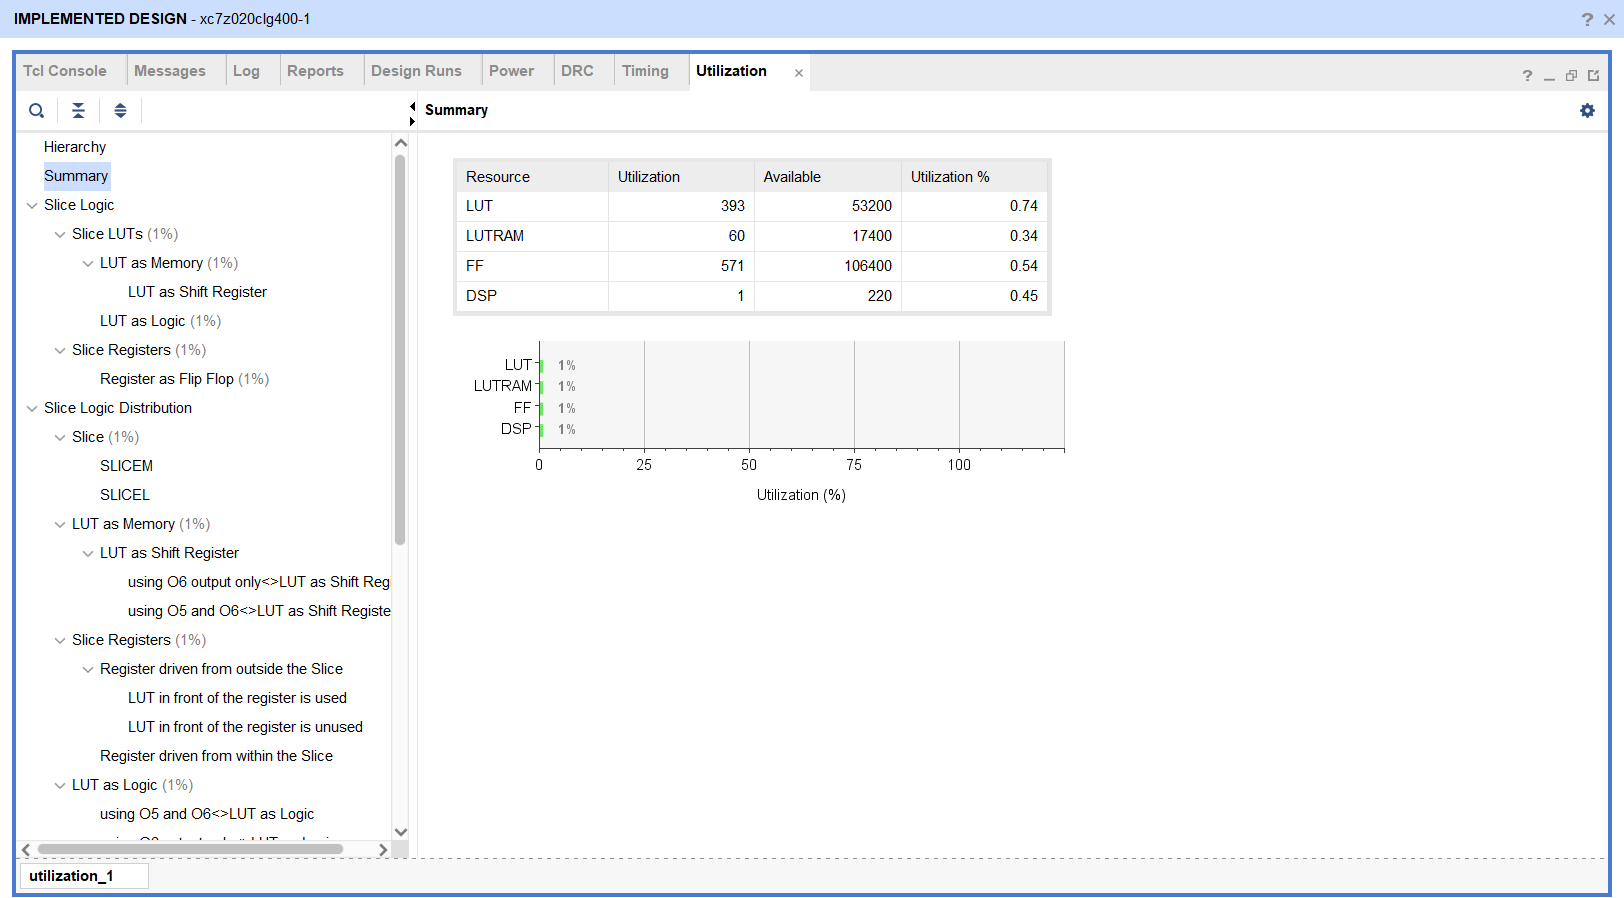
\includegraphics[width=14cm]{6_new.png}
    \caption{Resource Utilization Report of Multiplier}
    \label{fig:6}
\end{figure}
The resource utilization report is shown in picture above. Specifically, the multiplier uses 49 LUTs, 138 FFs and 1 DSP. Generally, this design is reasonable with compact logic (small number of LUTs); but the number of FF is a bit large, which may be used to satisfy timing issues. 
%\\\hspace*{\fill}\\

\begin{figure}[H]
    \centering
    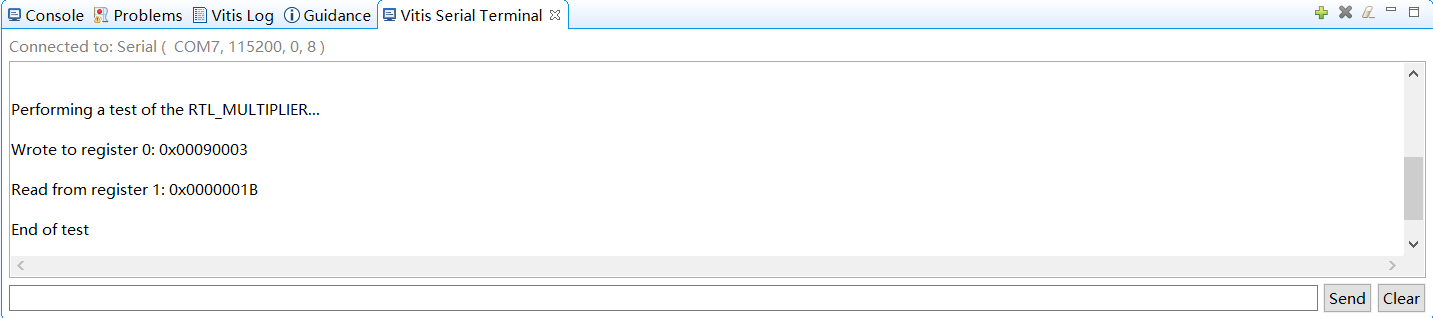
\includegraphics[width=14cm]{7_new.png}
    \caption{Screenshot of your SDK Terminal for the multiplier}
    \label{fig:7}
\end{figure}

\begin{figure}[H]
    \centering
    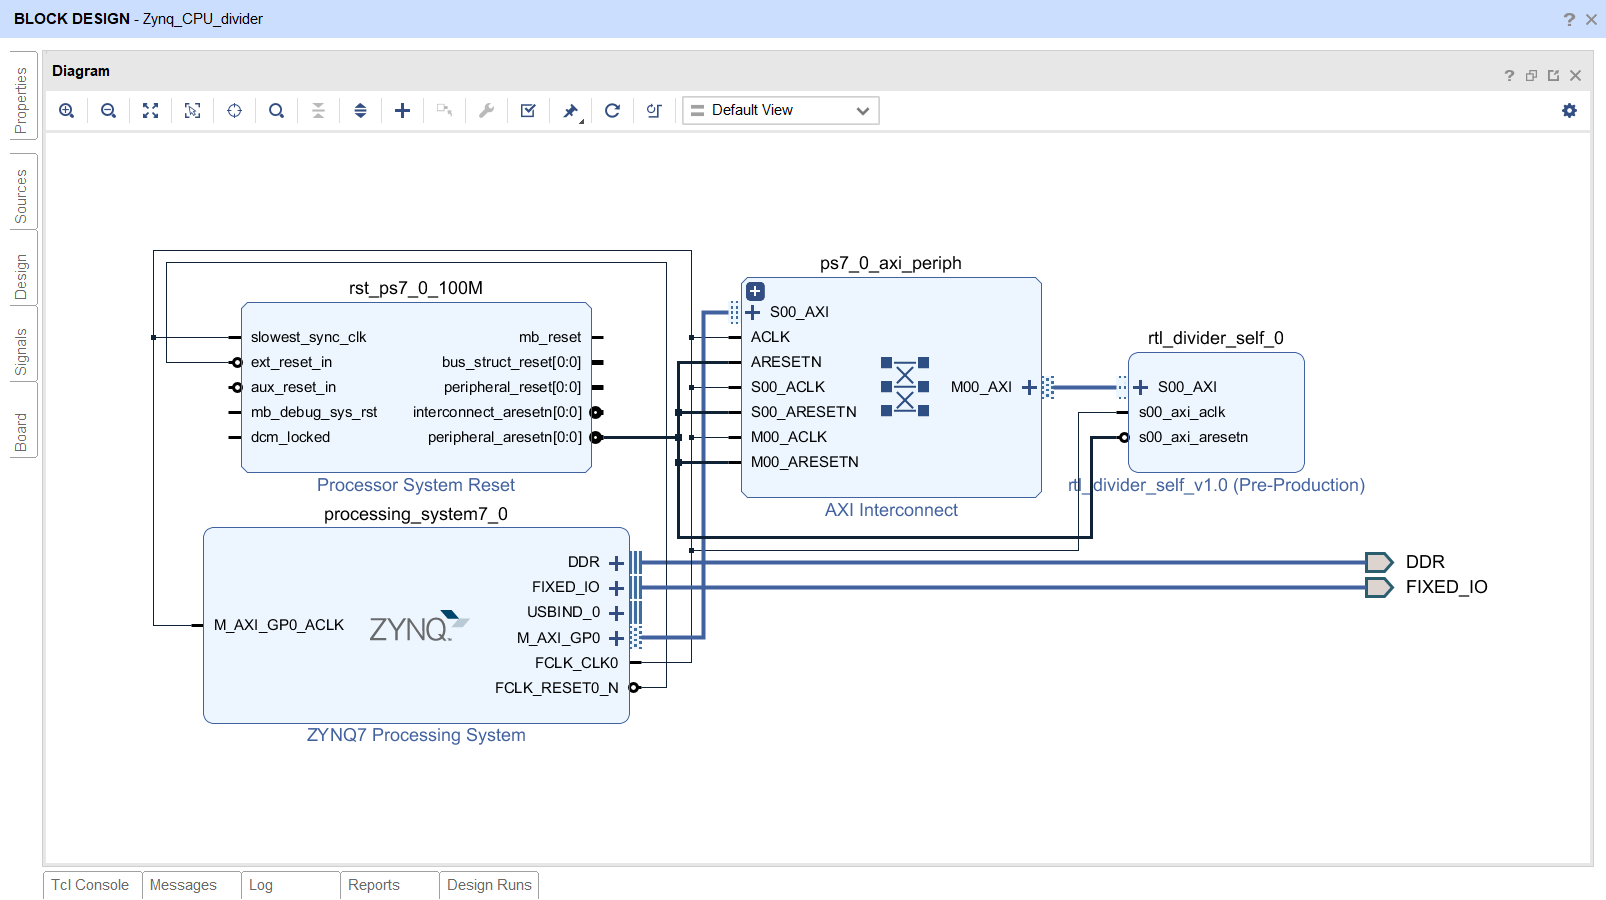
\includegraphics[width=14cm]{8}
    \caption{Screenshot of the Divider}
    \label{fig:8}
\end{figure}

\begin{figure}[H]
    \centering
    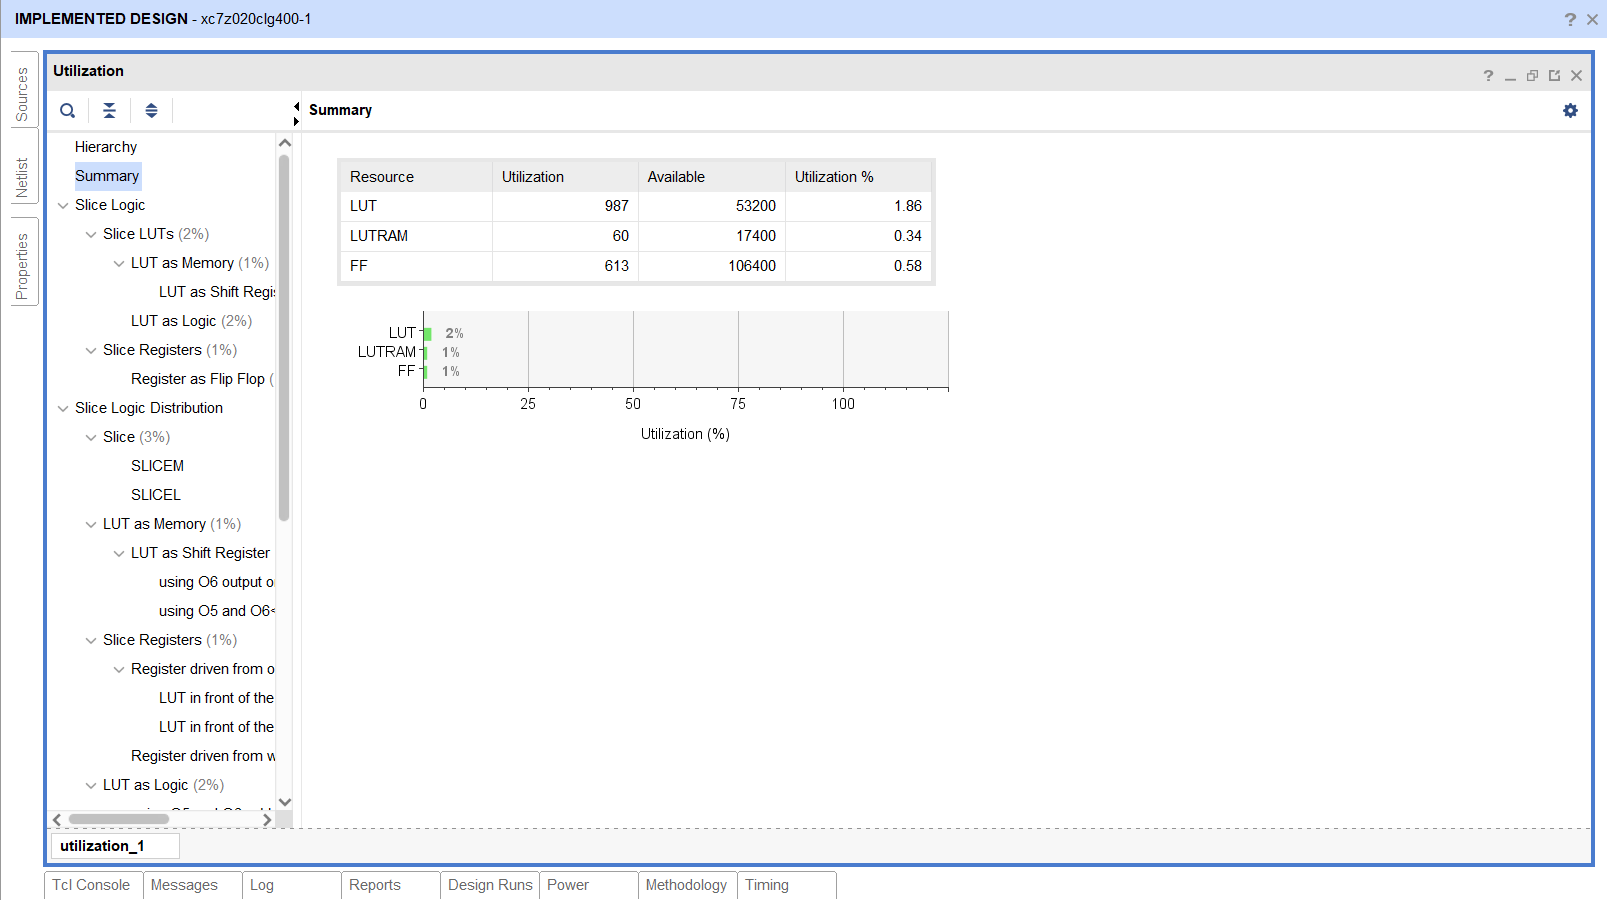
\includegraphics[width=14cm]{9}
    \caption{Resource Utilization Report of the Divider}
    \label{fig:9}
\end{figure}
The resource utilization report of our divider is shown in the picture above. Specifically, the divider uses 403 LUTs, and 32 FFs. The number of LUTs seems too large, which indicates the logic might be simplied. The number of flip-flops is reasonable. 

\begin{figure}[H]
    \centering
    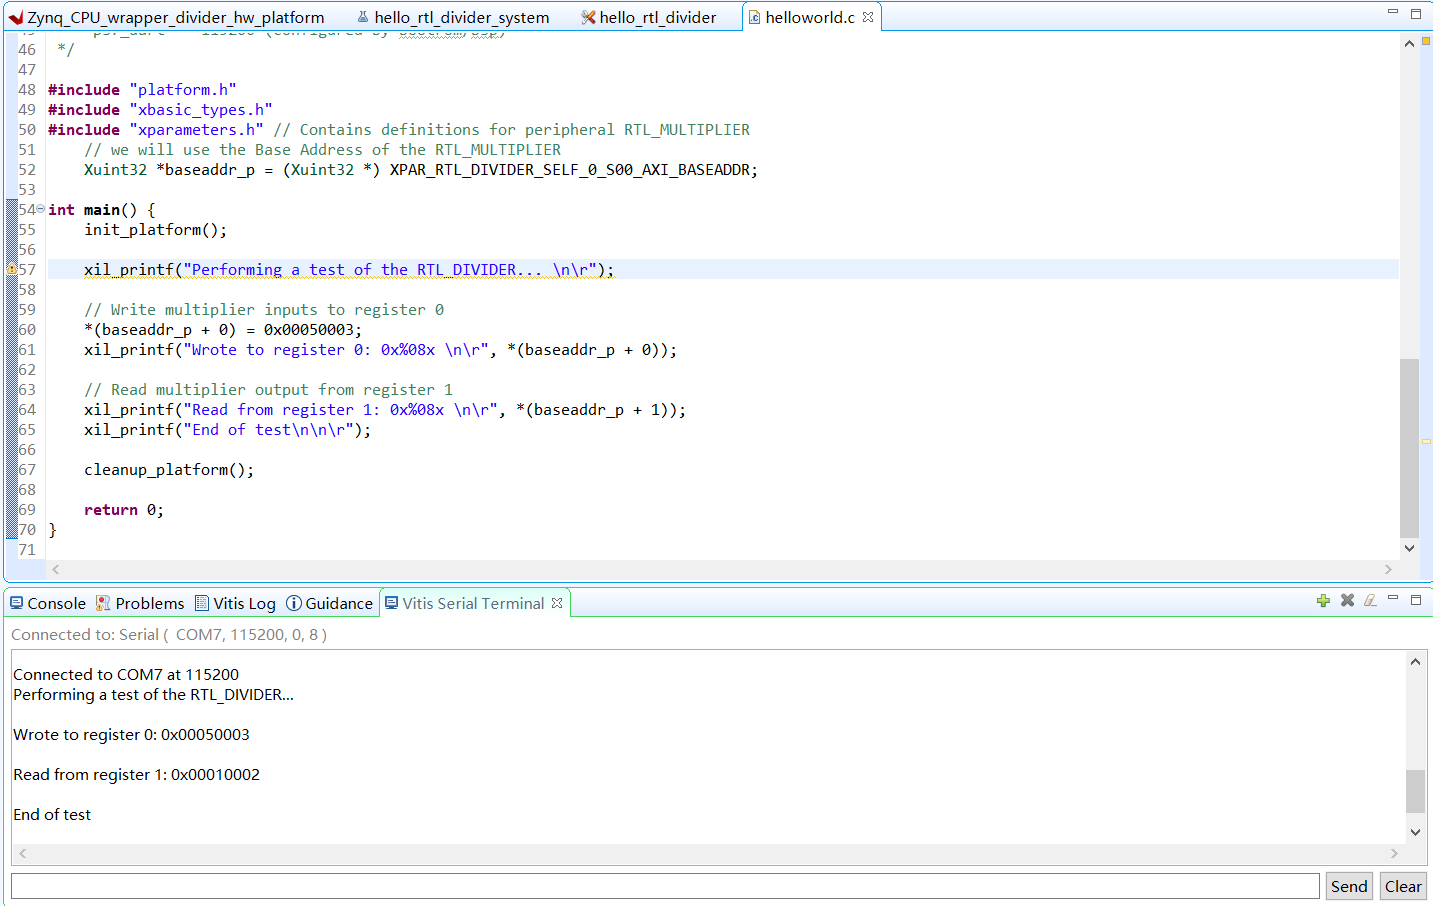
\includegraphics[width=14cm]{10_new.png}
    \caption{Screenshot of SDK Terminal for the Divider}
    \label{fig:10}
\end{figure}
For this divider, we also input two 16-bit numbers, whose concatenation corresponding to register 0. The output is the quotient and the remainder, both are also 16-bit, since if we assume both input numbers as integers, the remainder will be smaller than the divisor and the qoutient will be smaller than the dividend.
\begin{figure}[H]
    \centering
    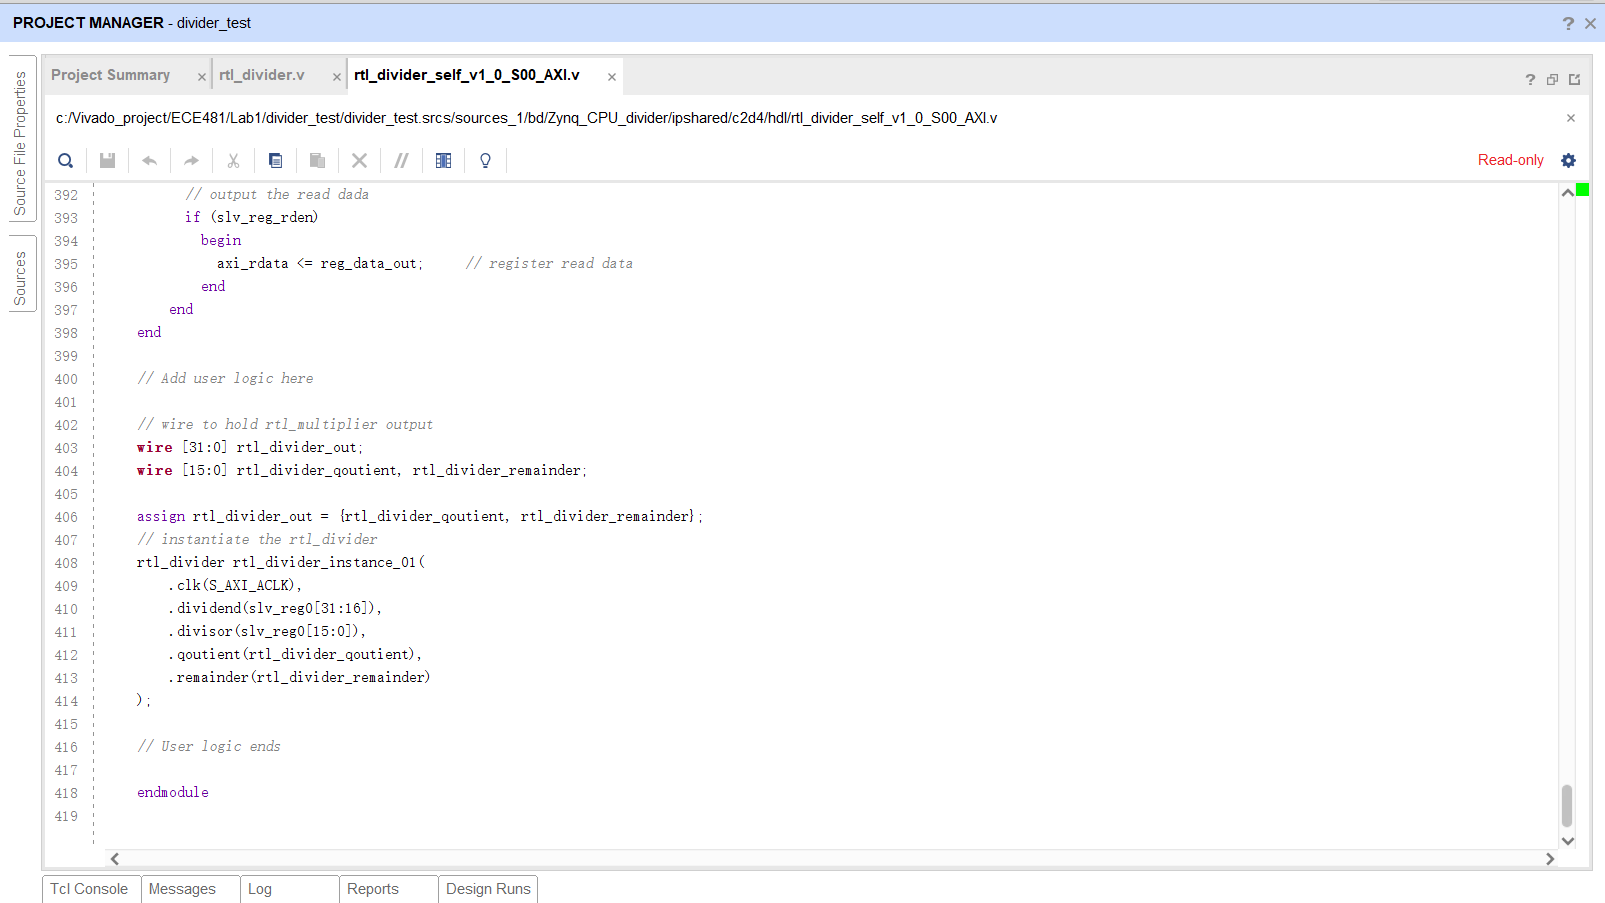
\includegraphics[width=14cm]{11}
    \caption{Connection between the divider and AXI registers}
    \label{fig:11}
\end{figure}

\begin{figure}[H]
    \centering
    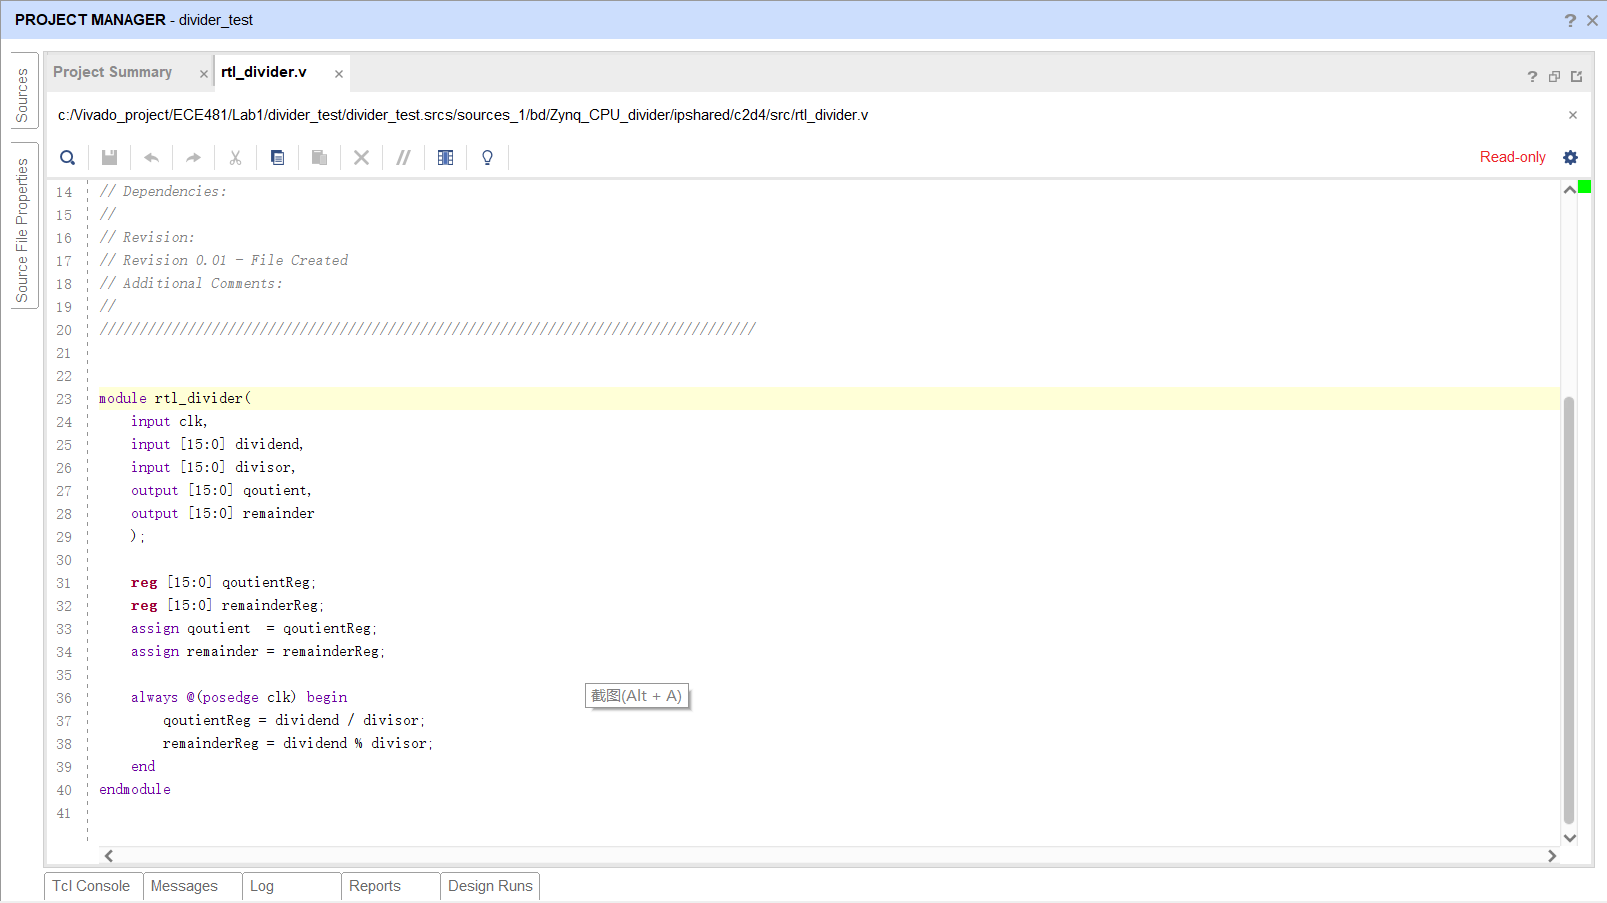
\includegraphics[width=14cm]{12}
    \caption{The Divider Source Code (Verilog)}
    \label{fig:12}
\end{figure}
The screenshot of the divider module is shown above. The code file is submitted together with this report in the zip package.
\clearpage
\section{Answer the Questions}
1.What is a bare metal test?
\par
"bare metal" means that the computer purely combined with hardware without operating system. A bare metal test is the test that tests the system or desired software feature directly without involving of operating system.
\par
2.How does the Zynq PS communicate with the IP blocks we created in this lab?
\par
The Zynq PS mainly communicate with the IP blocks, which we created in PL (programmable logic) part via AXI interface. For instance, the multiplier/divider IP block we created is connected to AXI-Lite interface as a slave. The input number is from the \textit{slv\_reg0}, and the module output is connected to \textit{slv\_reg1}. 
\par
3.Briefly read out the AXI, and summarize the main features.
\par
AXI means Advanced eXtensible Interface. It is a interconnection structure designed by ARM. It can support wide bandwidth and small latency design. Because it is a one-way channel, the number of gates is reduced and thus latency can be controlled. In our design, AXI interconnect is used to connect rtl\_multiplier\_v1.0 (Pre-Production), ZYNQ7 Processing System, and Processor System Reset. AXI standard is used to specify connections between the PS (Processing System) and PL (Programmable Logic). AXI Interconnects manages and directs traffic between attached AXI interfaces, and AXI Interfaces passes data, addresses, and hand-shaking signals between master and slave clients within the system [2]. The AXI protocol in particular exhibits the following key features [3]:
\begin{itemize}
    \item address/control phases are separate from data phases
    \item byte strobes enable unaligned data transfers
    \item burst-based transactions possible with only start address issued
    \item read and write data channels are separate allowing low-cost Direct Memory Access (DMA)
    \item multiple outstanding addresses can be issued
    \item transactions can be completed out-of-order
    \item register stages are easily added for timing closure
\end{itemize}
\par
4.Overall, what did you learn from this lab? Any difficulties?
\par
As a short conclusion, we learned how to build a Vivado project including Zynq PS system and export the hardware part as a platform in Vitis. Also, we learned how to use Vitis IDE for design on a specific hardware, and how to use serial communication with FPGA board on Vitis. More importantly, we learned how to design and package our own IP blocks, how to connect it to AXI interface, and how to test the new IP block on FPGA board
\par
One major difficuly we meet in this lab is how to run C program using Vitis IDE on FPGA board, since the operations on Vitis is different from SDK on the lab instruction, we cannot follow the instructions directly. After taking a long time searching online, finally we found out the correct steps to build a project on Vitis and run it on the hardware.
\section{Reference}
[1] ECE4810J Lab\#1 instructions.

[2] The Zynq Book: Embedded Processing with the ARM$^\circledR$ Cortex$^\circledR$-A9 on the Xilinx$^\circledR$ Zynq$^\circledR$-7000 All Programmable SoC.

[3] ARM, “Introduction — Channel Definition” in \textit{AMBA AXI Protocol Specification}, v1.0, June 2003.
\end{document}
